\documentclass[10pt,a4paper]{article}
\usepackage[latin1]{inputenc}
\usepackage{amsmath}
\usepackage{amsfonts}
\usepackage{amssymb}
\usepackage{graphicx}
\usepackage{fullpage}
\usepackage{float}
\usepackage{listings}

\title{DD2424 Lab 3}
\author{Artem Los (arteml@kth.se)}
\date{\today}

\begin{document}

\maketitle

\section*{K Layer Networks with Batch Normalization}

\subsection*{Gradient check}
Instead of checking the gradients numerically, we used the assumption that if gradients are correct means we should be able to overfit the data and vice versa (this is influenced by the observations in the previous lab, i.e. when gradients were wrong, the accuracy was never higher than $10\%$). We also tested compared the results with assignment 2.

To test gradients, we set the goal to overfit the classifier on 100 samples using 100 epochs, a batch number of 100 and learning rate of $0.01$. The final accuracy on training set was $0.95$ for a two-layer network and $0.61$ for a three layer network. Thus, the gradients should be correct. Later tests confirm this (once better hyper-paramters were found).

\subsection*{Three layer network with and without batch norm}

\begin{figure}[H]
	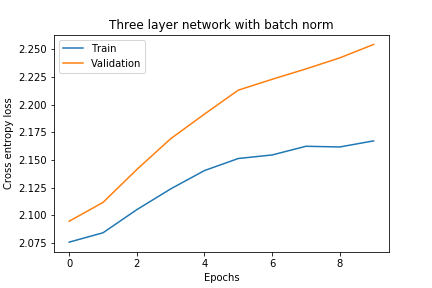
\includegraphics[width=7.5cm]{res/part2-with-bn.png}
	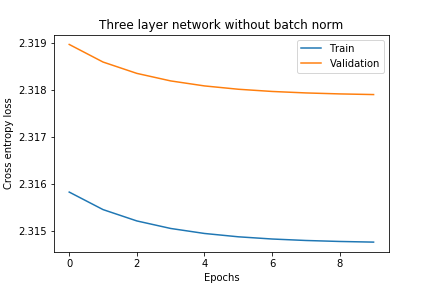
\includegraphics[width=7.5cm]{res/part2-without-bn.png}
	\caption{Training and validation errors when a 3 layer network was trained with \& without batch norm.}
\end{figure}

\subsection*{Best classifier}
When performing fine search, we used 3 epochs and $\eta=[10^{-2},10^{1}], \lambda=[10^{-5},10^{-4}]$. As a result, the best classifier obtained $\eta = 0.128729289, \lambda=1.55476073\times10^{-5}$ with $0.4252$ test accuracy.

\subsection*{Two layer network with differenent learning rates}
The plots below illustrate evolutions of the error for different learning rates. High, medium and small are 0.1, 0.01 and 0.01 respectively.

\begin{figure}[H]
	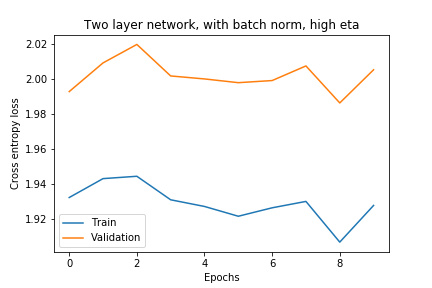
\includegraphics[width=5cm]{res/part4-bn_high.png}
	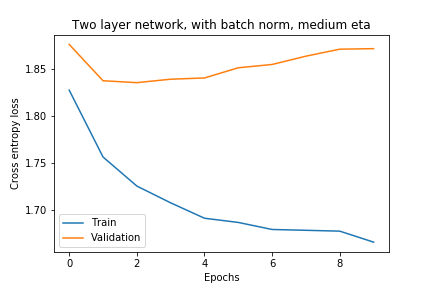
\includegraphics[width=5cm]{res/part4-bn_medium.png}
	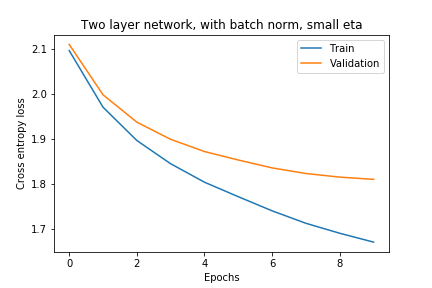
\includegraphics[width=5cm]{res/part4-bn_small.png}
	\\
	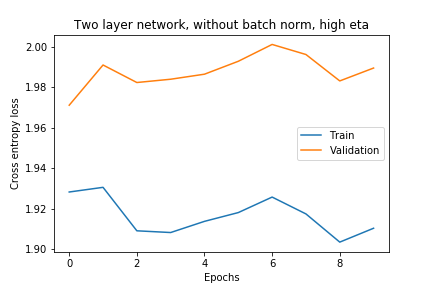
\includegraphics[width=5cm]{res/part4-nobn_high.png}
	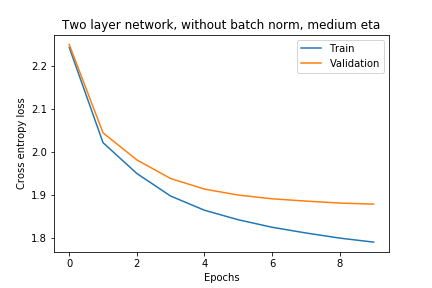
\includegraphics[width=5cm]{res/part4-nobn_medium.png}
	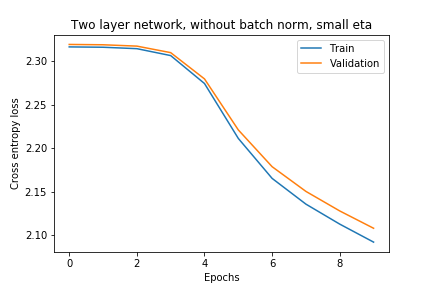
\includegraphics[width=5cm]{res/part4-nobn_small.png}
	\caption{Evolution of two layer network for different learning rates and constant lambda. The top raw
	is with batch normalization and the bottom row is without.}
\end{figure}

\end{document}